\documentclass[12pt]{article}
\usepackage{amsmath}
\usepackage{array}
% \usepackage{gensymb}
\usepackage{geometry}
\usepackage{graphicx}
\usepackage{pgfplots}
\usepackage{siunitx}
\usepackage{wrapfig}

\title{Homework \#8}
\author{Donald Aingworth IV}
\date{October 16, 2024}

\pgfplotsset{width=8cm,compat=1.9}
\usepgfplotslibrary{external}
% \tikzexternalize

\begin{document}

\DeclareSIUnit{\mile}{mi}
\DeclareSIUnit{\gal}{gal}
\DeclareSIUnit{\foot}{ft}
\DeclareSIUnit{\h}{h}

\maketitle

\pagebreak
\section*{Problem 1}
A 0.315-kg particle moves from an initial position $\vec{r}_1$ = $2.00 \hat{i} - 1.00 \hat{j} + 3.00 \hat{k}$ m to a final position $\vec{r}_2 = 4.00 \hat{i} - 3.00 \hat{j} - 1.00 \hat{k}$ m while a force $\vec{F} = 2.00 \hat{i} - 3.00 \hat{j} + 1.00 \hat{k}$ N acts on it. What is the work done by the force on the particle?

\subsection*{Solution}
We know the formula for work is $W = \vec{F} \cdot \vec{d}$. We can then apply the change in position for the distance traveled. We can then substitute in values to find the answer.
\begin{align*}
    \vec{d} &= \vec{r_2} - \vec{r_1}\\
            &= (4.00 \hat{i} - 3.00 \hat{j} - 1.00 \hat{k}) - (2.00 \hat{i} - 1.00 \hat{j} + 3.00 \hat{k})\ \unit{\meter}\\
            &= 2.00 \hat{i} - 2.00 \hat{j} - 4.00 \hat{k}\ \unit{\meter}\\
    W   &= \vec{F} \cdot \vec{d}\\
        &= (2.00 \hat{i} - 3.00 \hat{j} + 1.00 \hat{k}\ \unit{\newton}) \cdot (2.00 \hat{i} - 2.00 \hat{j} - 4.00 \hat{k}\ \unit{\meter})\\
        &= 2*2 + (-3)*(-2) + 1*(-4)\ \unit{\joule} 
        = (4 + 6 - 4)\ \unit{\joule}
        = \boxed{ 6\ \unit{\joule} }
\end{align*}

\pagebreak
\section*{Problem 2}
Compute the kinetic energy for each of the cases below. Through what distance would a 800-N force have to act to stop each object? (a) A 150-g baseball moving at 40 m/s; (b) a 13-g bullet from a rifle moving at 635 m/s; (c) a 1500-kg Corvette moving at 250 km/h; (d) a $1.8 \times 10^5$ kg Concorde airliner moving at 2240 km/h.


\subsection*{Solution}
In every case, we start with the formula of the work-kinetic energy thorem. We then substitute in formulae for work and kinetic energy, keeping in mind that the final velocity is zero (so the final kinetic energy $K_f = \frac{1}{2}mv_f^2$ is zero). We also keep in mind that the force would be applied in a direction opposite the kinetic energy.
\begin{align*}
    W   &= K_f - K_i\\
    F \cdot d   &= \frac{1}{2}mv_f^2 - \frac{1}{2}mv_i^2\\
    d   &= \frac{-\frac{1}{2}mv_i^2}{F}
\end{align*}

\subsubsection*{Section (a)}
\begin{align*}
    K   &= \frac{1}{2}mv^2 = \frac{1}{2} 0.15 * 40^2 = \boxed{120 \unit{\joule}}\\
    d   &= \frac{-\frac{1}{2}0.15*40^2 \unit{\joule}}{-800 \unit{\newton}}
        = \frac{0.15 * 800}{800} \unit{\meter} 
        = \boxed{0.15 \unit{\meter}}
\end{align*}

\subsubsection*{Section (b)}
\begin{align*}
    K   &= \frac{1}{2}mv^2 = \frac{1}{2} 0.013 * 635^2 = \boxed{2621 \unit{\joule}}\\
    d   &= \frac{-\frac{1}{2}0.013*635^2 \unit{\joule}}{-800 \unit{\newton}}
        = \frac{0.013 * 403225}{1600} \unit{\meter} 
        = \boxed{3.28 \unit{\meter}}
\end{align*}

\subsubsection*{Section (c)}
\begin{align*}
    v_i &= 250 \unit{\kilo\meter/\hour} * \frac{1000 \unit{\meter}}{1 \unit{\kilo\meter}} * \frac{1 \unit{\hour}}{3600 \unit{\second}} = \frac{625}{9} \unit{\meter/\second}\\
    K   &= \frac{1}{2}mv^2 = \frac{1}{2} 1500 * \frac{625}{9}^2 = \boxed{3616898 \unit{\joule}}\\
    d   &= \frac{-\frac{1}{2}1500*\frac{625}{9}^2 \unit{\joule}}{-800 \unit{\newton}}
        = \frac{1500*\frac{390625}{81}}{1600} \unit{\meter} 
        = \boxed{\frac{1953125}{432} \unit{\meter} = 4521 \unit{\meter}}
\end{align*}

\subsubsection*{Section (d)}
\begin{align*}
    v_i &= 2240 \unit{\kilo\meter/\hour} * \frac{1000 \unit{\meter}}{1 \unit{\kilo\meter}} * \frac{1 \unit{\hour}}{3600 \unit{\second}} = \frac{5600}{9} \unit{\meter/\second}\\
    K   &= \frac{1}{2}mv^2 = \frac{1}{2} 1.8*10^5 * \frac{5600}{9}^2 = \boxed{3.484 \times 10^{10} \unit{\joule}}\\
    d   &= \frac{-\frac{1}{2}1.8*10^5*\frac{5600}{9}^2 \unit{\joule}}{-800 \unit{\newton}}
        = \frac{1.8*10^9*\frac{3136}{81}}{1600} \unit{\meter} 
        = \boxed{\frac{39200000000}{9} \unit{\meter} = 4.36 \times 10^9 \unit{\meter}}
\end{align*}

\pagebreak
\section*{Problem 3}
Compute the kinetic energies for each of the following. What force would be required to stop each object in 1.00 km? (a) The $8.00 \times 10^7 \unit{\kilo\gram}$ carrier Nimitz moving at 55 km/h; (b) a $3.4 \times 10^5 \unit{\kilo\gram}$ Boeing 747 moving at 1000 km/h; (c) the 270-kg Pioneer 10 spacecraft moving at 51,800 km/h.

\subsection*{Solution}
In every case, we start with the formula of the work-kinetic energy thorem. We then substitute in formulae for work and kinetic energy, keeping in mind that the final velocity is zero (so the final kinetic energy $K_f = \frac{1}{2}mv_f^2$ is zero). We also keep in mind that the force would be applied in a direction opposite the kinetic energy.
\begin{align*}
    K_i &= \frac{1}{2}mv_i^2\\
    F \cdot d = W   &= K_f - K_i = \frac{1}{2}mv_f^2 - \frac{1}{2}mv_i^2\\
    F   &= \frac{-\frac{1}{2}mv_i^2}{d}
\end{align*}

\subsubsection*{Section (a)}
\begin{align*}
    v   &= 55 \unit{\kilo\meter/\hour} * \frac{1000\ \unit{\meter*\hour}}{3600\ \unit{\kilo\meter*\second}} 
        = \frac{275}{18} \unit{\meter/\second}\\
    K_i &= \frac{1}{2}mv_i^2 
        = \frac{1}{2} * 8.00 \times 10^7 \unit{\kilo\gram} * \left( \frac{275}{18} \unit{\meter/\second} \right)^2 
        = 9.34 \times 10^9 \unit{\joule}\\
    F   &= \frac{-\frac{1}{2}mv_i^2}{d}
        = \frac{-9.34 \times 10^9 \unit{\joule}}{1000 \unit{\meter}}
        = -9.34 \times 10^6 \unit{\newton}
\end{align*}
This means that the kinetic energy of the Nimitz is \boxed{9.34 \times 10^9 \unit{\joule}} in one direction, while the force required would be \boxed{9.34 \times 10^6 \unit{\newton}} in the opposite direction.

\pagebreak
\subsubsection*{Section (b)}
\begin{align*}
    v   &= 1000 \unit{\kilo\meter/\hour} * \frac{1000\ \unit{\meter*\hour}}{3600\ \unit{\kilo\meter*\second}} 
        = \frac{2500}{9} \unit{\meter/\second}\\
    K_i &= \frac{1}{2}mv_i^2 
        = \frac{1}{2} * 3.40 \times 10^5 \unit{\kilo\gram} * \left( \frac{2500}{9} \unit{\meter/\second} \right)^2 
        = 1.31 \times 10^{10} \unit{\joule}\\
    F   &= \frac{-\frac{1}{2}mv_i^2}{d}
        = \frac{-1.31 \times 10^10 \unit{\joule}}{1000 \unit{\meter}}
        = -1.31 \times 10^7 \unit{\newton}
\end{align*}
This means that the kinetic energy of the Boeing 747 is \boxed{1.31 \times 10^{10} \unit{\joule}} in one direction, while the force required would be \boxed{1.31 \times 10^7 \unit{\newton}} in the opposite direction.

\subsubsection*{Section (c)}
\begin{align*}
    v   &= 51800 \unit{\kilo\meter/\hour} * \frac{1000\ \unit{\meter*\hour}}{3600\ \unit{\kilo\meter*\second}} 
        = \frac{129500}{9} \unit{\meter/\second}\\
    K_i &= \frac{1}{2}mv_i^2 
        = \frac{1}{2} * 270.0 \unit{\kilo\gram} * \left( \frac{129500}{9} \unit{\meter/\second} \right)^2 
        = 2.80 \times 10^{10} \unit{\joule}\\
    F   &= \frac{-\frac{1}{2}mv_i^2}{d}
        = \frac{-2.80 \times 10^{10} \unit{\joule}}{1000 \unit{\meter}}
        = -2.80 \times 10^7 \unit{\newton}
\end{align*}
This means that the kinetic energy of the Pioneer 10 is \boxed{2.80 \times 10^{10} \unit{\joule}} in one direction, while the force required would be \boxed{2.80 \times 10^7 \unit{\newton}} in the opposite direction.

\pagebreak
\section*{Problem 4}

\begin{wrapfigure}{r}{0.25\textwidth}
    \vspace{-25pt}
    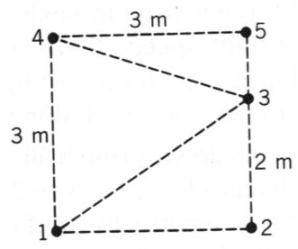
\includegraphics[width=0.25\textwidth]{graph_4.png} 
\end{wrapfigure}
A 1.50-kg block is moved at constant speed in a vertical plane from position 1 to position 3 via several routes shown in the figure. Compute the work done by gravity on the block for each segment indicated, where $W_{ab}$ means work done from a to b. (a) $W_{13}$, (b) $W_{12}$ + $W_{23}$ (c) $W_{14}$ + $W_{43}$, (d) $W_{14}$ + $W_{45}$ + $W_{53}$.

\subsection*{Solution}
For each section, we use the formula of gravitational work, which is \( W_g = m g d \cos(\phi) \), $\phi_g$ being the angle between the vertical force of gravity and the motion itself. We can derive from the cosine ratio (SOH\textbf{CAH}TOA) that $\cos(\phi) = \frac{\text{height}}{\text{distance}} = \frac{h}{d}$. Applying this to the formula for work, we get $W_g = mgh$. 

\subsubsection*{Section (a)}
\begin{align*}
    W_{13}  &= mg(h_3 - h_1) 
            = 1.50 * -9.81 * (2 - 0) \unit{\joule} 
            = \boxed{ -29.43\unit{\joule} }
\end{align*}

\subsubsection*{Section (b)}
\begin{align*}
    W_{12} + W_{23} &= mg(h_2 - h_1) + mg(h_3 - h_2)\\
        &= 1.50 * -9.81 * (0 - 0) \unit{\joule} + 1.50 * -9.81 * (2 - 0) \unit{\joule} 
        = \boxed{ -29.43\unit{\joule} }
\end{align*}

\subsubsection*{Section (c)}
\begin{align*}
    W_{14} + W_{43} &= mg(h_4 - h_1) + mg(h_3 - h_4)\\
        &= 1.50 * -9.81 * (3 - 0) \unit{\joule} + 1.50 * -9.81 * (2 - 3) \unit{\joule}\\
        &= 4.5 * -9.81 - 1.5 * -9.81 = 3.0 * -9.81 
        = \boxed{ -29.43\unit{\joule} }
\end{align*}

\subsubsection*{Section (d)}
\begin{align*}
    W_{14} + W_{45} + W_{53} &= mg(h_4 - h_1) + mg(h_5 - h_4) + mg(h_3 - h_5)\\
        &= 1.50 * g * (3 - 0) \unit{\joule} + 1.50 * g * (3 - 3) \unit{\joule} + 1.50 * g * (2 - 3) \unit{\joule}\\
        &= 1.50 * -9.81 * 2\ \unit{\joule} = \boxed{ -29.43\unit{\joule} }
\end{align*}


\pagebreak
\section*{Problem 5}
What is the work needed to lift 14.7 kg of water from a well 11.0 m deep. Assume the water has a constant upward acceleration of 0.700 m/s$^2$.

\subsection*{Solution}
Here, the net force is equal to the gravitational force plus the applied force. We can then use the work formulae.
\begin{align*}
    F_{net} = 
    ma  &=  F_{app} + F_g = F_{app} - m*9.81\unit{\meter/\second^2}\\
    F_{app} &= m(a + 9.81\unit{\meter/\second^2}) - 14.7(0.7 + 9.81)\unit{\newton}
            = 154.497 \unit{\meter/\second^2}\\
    W   &=  154.497 * 11 = \boxed{1699.497\unit{\joule}}
\end{align*}

\pagebreak
\section*{Problem 6}

\begin{wrapfigure}{r}{0.25\textwidth}
    \vspace{-50pt}
    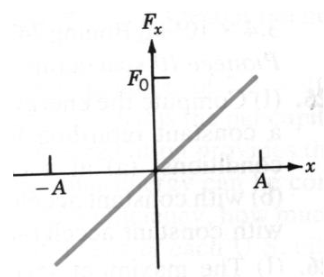
\includegraphics[width=0.25\textwidth]{graph_6.png} 
    % \label{fig:wrapfig}
\end{wrapfigure}
The variation of a force with position is shown in the figure below. Find the work from (a) x = 0 to x = -A (b) x = +A to x = 0

\subsection*{Solution}
a) $\frac{1}{2}F_0 A$\\
We here use the integral for work along a curve.
\begin{align*}
    F(x)    &=  \frac{F_0}{A} x\\
    W_1 &= \int_{x_i}^{x_f} F(x) dx 
        = \int_0^{-A} \frac{F_0}{A}x\ dx 
        = \left(\frac{F_0}{2A}x^2\right)_0^{-A} 
        = \frac{F_0 (-A)^2}{2A} = \boxed{\frac{F_0 A}{2}}
\end{align*}

b)$-\frac{F_0 A}{2}$\\
We use the same thng here.
\begin{align*}
    W_2 &= \int_{x_i}^{x_f} F(x) dx 
        = \int_A^0 \frac{F_0}{A}x\ dx 
        = \left(\frac{F_0}{2A}x^2\right)_A^0 
        = -\frac{F_0 (-A)^2}{2A} = \boxed{-\frac{F_0 A}{2}}
\end{align*}

\pagebreak
\section*{Problem 7}

Consider a particle on which several forces act, one of which is known to be constant in time: $\vec{F}_1$ = 3.00 $\hat{i}$ + 4.00 $\hat{j}$ N. As a result, the particle moves along a straight path from a Cartesian coordinate of (0.00 m, 0.00 m) to (5.00 m, 6.00 m). What is the work done by $\vec{F}_1$?

\subsection*{Solution}
We here use the dot product.
\begin{align*}
    W   &=  \vec{F} \cdot \vec{d}
        =   \begin{pmatrix} 3 \unit{\newton} \\ 4 \unit{\newton} \end{pmatrix} \cdot \begin{pmatrix} 5 \unit{\meter} \\ 6 \unit{\meter} \end{pmatrix}
        =   3 * 5 + 4 * 6 \ \unit{\joule}
        =   15 + 24 \ \unit{\joule} = \boxed{39 \unit{\joule}}
\end{align*}

\pagebreak
\section*{Problem 8}
A bungee cord exerts a nonlinear elastic force of magnitude $F(x) = k_1x + k_2 x^3$, where $x$ is the distance the cord is stretched, $k_1 = 204 \unit{\N/\m}$ and $k_2 = -0.233 \unit{\N/\m^3}$. How much work must be done on the cord to stretch
it 16.7 m?

\subsection*{Solution}
We here use the integral for work doen by a spring.
\begin{align*}
    W_s &=  \int_{x_i}^{x_f} F_x\ dx
        =   \int_{0}^{16.7} k_1 x + k^2 x^3\ dx
        =   \int_{0}^{16.7} 204x - 0.233x^3\ dx\\
        &=  \left(\frac{204x^2}{2} - \frac{0.233x^4}{4}\right)_0^{16.7}
        =   \left(102 16.7^2 - \frac{0.233*16.7^4}{4}\right) \unit{\joule}\\
        &=  \boxed{23916.116 \unit{\joule}}
\end{align*}


\end{document}